\documentclass{standalone}
\usepackage{mintikz}

\begin{document}
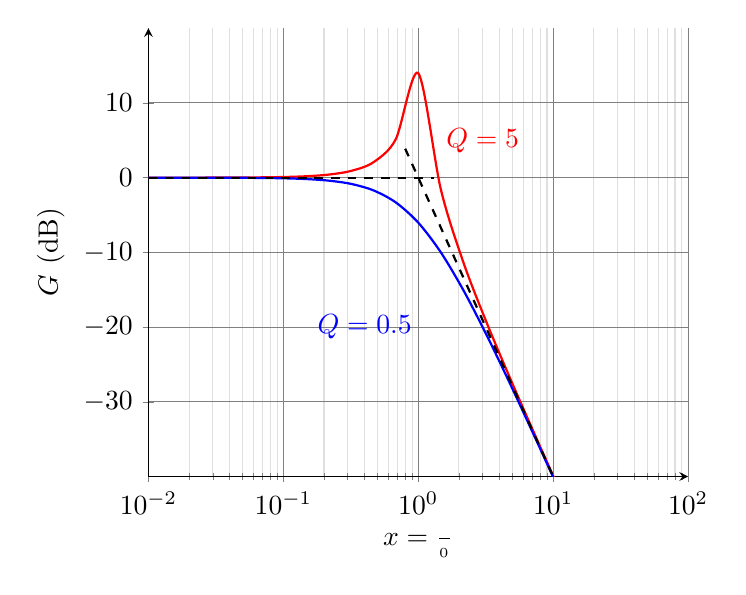
\begin{tikzpicture}[]
    \begin{semilogxaxis}[
        xmin=1e-2, xmax=1e2,
        ymin=-40, ymax=20,
        xlabel={$x=\DS\frac{\w}{\w_0}$}, ylabel=$G_{\dB}$ (dB),
        ytick={-30, -20, ..., 10},
        axis lines=left,
        grid=both,
        major grid style={black!50},
        minor grid style={gray!25},
        clip=true]
        \def\Q{5}
        \addplot[
        domain=1e-2:1e2,
        smooth, thick, red]
        %{log10(\x)};
        {-10*log10((1-\x^2)^2+(\x/\Q)^2)};
        \def\Q{.5}
        \addplot[
        domain=1e-2:1e2,
        smooth, thick, blue]
        %{log10(\x)};
        {-10*log10((1-\x^2)^2+(\x/\Q)^2)};
        \addplot[
        domain=1e-2:1.3,
        smooth, black, dashed, thick]
        {0};
        \addplot[
        domain=8e-1:1e2,
        smooth, black, dashed, thick]
        {-40*log10(\x)};
        \node[color=red] at (axis cs:3,5) {$Q=5$};
        \node[color=blue] at (axis cs:.4,-20) {$Q=0.5$};
        % \draw[dashed, thick]
        % (axis cs:1e-2,-3) -|
        % (axis cs:1e0,-30);
    \end{semilogxaxis}
\end{tikzpicture}
\end{document}
